% NE 630 -- Chapter 4 reading-guide shared definitions, Lessons 15--18
% Included by lesson_15_handout.tex through lesson_18_handout.tex.
% Layout/palette adapted from the user's ne630boardhandout class.
% Content: supplied chapter(1).tex and lecture_15.tex through lecture_19.tex.
% The supplied chapter numbers the four-factor discussion as Section 4.5.
% Drawings below adapt supplied Fig. 4.1, Fig. 4.5, Fig. 4.6, and the L19
% pin-cell drawing. They are qualitative schematics, not simulation results.
\documentclass[10pt,letterpaper]{article}
\usepackage{amsmath,mathtools}
\usepackage{libertinus,microtype}
\usepackage[left=0.48in,right=0.48in,top=0.48in,bottom=0.44in,
  headheight=20pt,headsep=5pt,footskip=17pt,includeheadfoot]{geometry}
\usepackage{graphicx,xcolor,tabularx,booktabs,array,ragged2e}
\usepackage{tikz}
\usetikzlibrary{arrows.meta,calc,positioning,patterns}
\usepackage[most]{tcolorbox}
\usepackage{fancyhdr,lastpage}
\usepackage[hidelinks]{hyperref}
\hypersetup{pdfauthor={NE 630},pdfsubject={The Power Reactor Core}}
\definecolor{KSUPurple}{HTML}{512888}
\definecolor{KSUDeepPurple}{HTML}{3B1B64}
\definecolor{KSUOrange}{HTML}{CA7C1B}
\definecolor{KSUGray}{HTML}{5D5D5D}
\setlength{\parindent}{0pt}
\setlength{\parskip}{3pt}
\setlength{\emergencystretch}{1.5em}
\setlength{\abovedisplayskip}{4pt}
\setlength{\belowdisplayskip}{4pt}
\setlength{\abovedisplayshortskip}{2pt}
\setlength{\belowdisplayshortskip}{3pt}
\setlength{\jot}{3pt}
\renewcommand{\arraystretch}{1.12}
\newcolumntype{Y}{>{\RaggedRight\arraybackslash}X}
\newcommand{\LessonNo}{15}
\pagestyle{fancy}
\fancyhf{}
\fancyhead[L]{\sffamily\bfseries\small NE 630}
\fancyhead[C]{\sffamily\small The Power Reactor Core}
\fancyhead[R]{\sffamily\bfseries\small Lesson \LessonNo}
\fancyfoot[L]{\sffamily\scriptsize  }
\fancyfoot[C]{\sffamily\scriptsize \thepage\ of \pageref*{LastPage}}
\fancyfoot[R]{\sffamily\scriptsize }
\renewcommand{\headrulewidth}{0.5pt}
\makeatletter
\renewcommand{\headrule}{\hbox to\headwidth{\color{KSUPurple}\leaders\hrule height .5pt\hfill}}
\makeatother
\newcommand{\Lesson}[4]{%
  \renewcommand{\LessonNo}{#1}%
  \noindent\begin{minipage}[c]{0.025\linewidth}\color{KSUPurple}\rule{3.5pt}{32pt}\end{minipage}%
  \begin{minipage}[c]{0.815\linewidth}
   {\sffamily\bfseries\fontsize{18}{20}\selectfont #2}\par
   {\sffamily\fontsize{9}{10.5}\selectfont #4}
  \end{minipage}\hfill
  \begin{minipage}[c]{0.14\linewidth}\raggedleft
    {\sffamily\color{KSUPurple}\bfseries\fontsize{25}{26}\selectfont #1}\par
    {\sffamily\scriptsize LESSON}
  \end{minipage}\par\vspace{3pt}
  \begin{tcolorbox}[enhanced,boxrule=.45pt,arc=1pt,colback=KSUPurple!4,
   colframe=KSUPurple!40,left=5pt,right=5pt,top=3pt,bottom=3pt,
   before skip=0pt,after skip=6pt]
   \sffamily\fontsize{9}{10.5}\selectfont\textbf{Read:} #3
  \end{tcolorbox}}
\newcommand{\Sec}[2]{\par\addvspace{5pt}\noindent
  \colorbox{KSUPurple}{\color{white}\sffamily\bfseries\fontsize{9}{10}\selectfont\strut #1}
  \hspace{3pt}{\sffamily\bfseries\color{KSUDeepPurple}\fontsize{10.2}{11.5}\selectfont #2}\par\vspace{1pt}}
\newcommand{\eqread}[1]{{\sffamily\fontsize{7.9}{9}\selectfont\color{KSUGray}#1}}
\newcommand{\figcap}[1]{\par\vspace{1pt}{\sffamily\fontsize{7.7}{9}\selectfont\color{KSUGray}#1}\par}
\newtcolorbox{KeyBox}[1]{enhanced,boxrule=.45pt,arc=1pt,
 colback=KSUPurple!3,colframe=KSUPurple!40,left=5pt,right=5pt,top=4pt,bottom=4pt,
 before skip=4pt,after skip=4pt,before upper=\RaggedRight,fonttitle=\sffamily\bfseries\small,
 coltitle=KSUDeepPurple,title={#1},colbacktitle=KSUPurple!7,
 titlerule=0pt,toptitle=2pt,bottomtitle=2pt}
\newtcolorbox{Explore}[1]{enhanced,boxrule=.5pt,arc=1pt,
 colback=KSUOrange!5,colframe=KSUOrange!65,left=6pt,right=6pt,top=4pt,bottom=4pt,
 before skip=7pt,after skip=3pt,before upper=\RaggedRight,
 title={OpenMC \enspace\textbar\enspace #1},fonttitle=\sffamily\bfseries\fontsize{9}{10}\selectfont,
 coltitle=KSUDeepPurple,colbacktitle=KSUOrange!10,titlerule=0pt,toptitle=2pt,bottomtitle=2pt}
\newcommand{\SourceLine}[1]{\par\vspace{2pt}{\sffamily\fontsize{7.2}{8.4}\selectfont\color{KSUGray}#1}\par}
\newcommand{\colstart}{\begin{minipage}[t]{.482\linewidth}\vspace{0pt}\RaggedRight}
\newcommand{\colnext}{\end{minipage}\hfill\begin{minipage}[t]{.482\linewidth}\vspace{0pt}\RaggedRight}
\newcommand{\colend}{\end{minipage}\par}
\newcommand{\uunit}[1]{\,\mathrm{#1}}
\newcommand{\metal}{\mathrm{metal}}
\newcommand{\water}{\mathrm{w}}
\newcommand{\fiiso}{\mathrm{fi}}
\newcommand{\feiso}{\mathrm{fe}}
\newcommand{\nucl}[2]{\ensuremath{{}^{#1}\mathrm{#2}}}



% Five reactor motifs, adapted from the supplied Fig. 4.1, with a compact TRISO zoom.
\newcommand{\FamilyFigure}{%
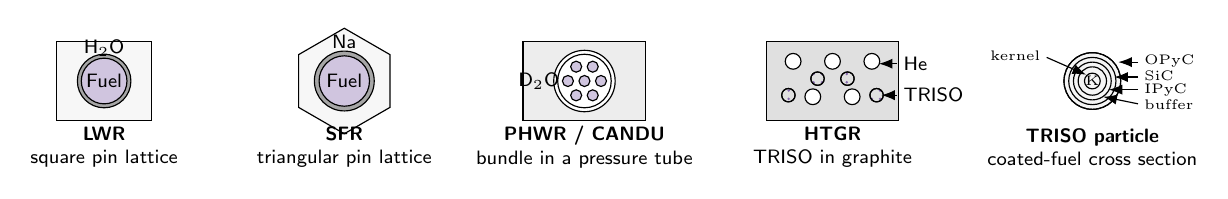
\begin{tikzpicture}[x=1cm,y=1cm,line width=.42pt,font=\sffamily\fontsize{7.5}{8.5}\selectfont,
 every node/.style={inner sep=1pt},>=Latex]
\begin{scope}[shift={(0,0)}]
 \draw[fill=black!3] (-.60,-.50) rectangle (.60,.50);
 \draw[fill=black!35] (0,0) circle (.34);
 \draw[fill=KSUPurple!27] (0,0) circle (.29);
 \node at (0,0) {Fuel}; \node at (0,.42) {H$_2$O};
 \node[align=center] at (0,-.84) {\textbf{LWR}\\square pin lattice};
\end{scope}
\begin{scope}[shift={(3.05,0)}]
 \draw[fill=black!3] (90:.67)--(30:.67)--(-30:.67)--(-90:.67)--(-150:.67)--(150:.67)--cycle;
 \draw[fill=black!35] (0,0) circle (.38);
 \draw[fill=KSUPurple!27] (0,0) circle (.32);
 \node at (0,0) {Fuel}; \node at (0,.50) {Na};
 \node[align=center] at (0,-.84) {\textbf{SFR}\\triangular pin lattice};
\end{scope}
\begin{scope}[shift={(6.10,0)}]
 \draw[fill=black!7] (-.78,-.50) rectangle (.78,.50);
 \draw[fill=white] (0,0) circle (.39);
 \draw (0,0) circle (.34);
 \foreach \ang in {0,60,...,300}{\draw[fill=KSUPurple!27] (\ang:.21) circle (.07);} 
 \draw[fill=KSUPurple!27] (0,0) circle (.07);
 \node[align=center] at (-.58,0) {D$_2$O};
 \node[align=center] at (0,-.84) {\textbf{PHWR / CANDU}\\bundle in a pressure tube};
\end{scope}
\begin{scope}[shift={(9.25,0)}]
 \draw[fill=black!12] (-.84,-.50) rectangle (.84,.50);
 \foreach \x/\y in {-.50/.25,0/.25,.50/.25,-.25/-.20,.25/-.20}{\draw[fill=white] (\x,\y) circle (.10);} 
 \foreach \x/\y in {-.56/-.18,-.19/.03,.19/.03,.56/-.18}{
   \draw[fill=KSUPurple!10,pattern=dots,pattern color=KSUPurple!70] (\x,\y) circle (.085);
   \draw (\x,\y) circle (.085);
 }
 \node[anchor=west] at (.86,.22) {He};
 \draw[->] (.82,.22)--(.59,.22);
 \node[anchor=west] at (.86,-.18) {TRISO};
 \draw[->] (.82,-.18)--(.62,-.18);
 \node[align=center] at (0,-.84) {\textbf{HTGR}\\TRISO in graphite};
\end{scope}
\begin{scope}[shift={(12.55,0)}]
 \draw[fill=KSUPurple!70] (0,0) circle (.10);  % kernel
 \draw[fill=KSUPurple!18] (0,0) circle (.18);  % buffer
 \draw[fill=gray!25] (0,0) circle (.24);       % inner PyC
 \draw[fill=green!12!black!8] (0,0) circle (.30); % SiC
 \draw[fill=gray!8] (0,0) circle (.36);        % outer PyC
 \foreach \r in {.10,.18,.24,.30,.36}{\draw (0,0) circle (\r);} 
 \node[font=\tiny] at (0,0) {K};
 \node[font=\tiny,anchor=west] at (.62,.25) {OPyC}; \draw[->] (.58,.24)--(.33,.24);
 \node[font=\tiny,anchor=west] at (.62,.06) {SiC};  \draw[->] (.58,.05)--(.28,.05);
 \node[font=\tiny,anchor=west] at (.62,-.12) {IPyC};\draw[->] (.58,-.11)--(.21,-.11);
 \node[font=\tiny,anchor=west] at (.62,-.30) {buffer};\draw[->] (.58,-.29)--(.14,-.20);
 \node[font=\tiny,anchor=east] at (-.62,.32) {kernel};\draw[->] (-.58,.30)--(-.08,.08);
 \node[align=center] at (0,-.84) {\textbf{TRISO particle}\\coated-fuel cross section};
\end{scope}
\end{tikzpicture}}

% Square and hexagonal pin cells, adapted from the L19 cell figure and Fig. 4.1.
\newcommand{\PinCellsFigure}{%
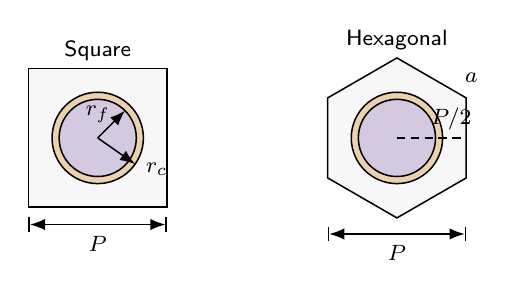
\begin{tikzpicture}[x=1cm,y=1cm,font=\sffamily\fontsize{8.5}{10}\selectfont,
 line width=.55pt,>=Latex,every node/.style={inner sep=1pt}]
\begin{scope}[shift={(0,0)}]
 \draw[fill=black!3] (-.88,-.88) rectangle (.88,.88);
 \draw[fill=KSUOrange!35] (0,0) circle (.58);
 \draw[fill=KSUPurple!25] (0,0) circle (.49);
 \draw[->] (0,0)--(45:.49) node[midway,above left=-1pt] {$r_f$};
 \draw[->] (0,0)--(-35:.58);\node[anchor=west] at (.57,-.40) {$r_c$};
 \draw[|<->|] (-.88,-1.10)--(.88,-1.10) node[midway,below=3pt] {$P$};
 \node at (0,1.10) {Square};
\end{scope}
\begin{scope}[shift={(3.80,0)}]
 \draw[fill=black!3] (90:1.016)--(30:1.016)--(-30:1.016)--(-90:1.016)--(-150:1.016)--(150:1.016)--cycle;
 \draw[fill=KSUOrange!35] (0,0) circle (.58);
 \draw[fill=KSUPurple!25] (0,0) circle (.49);
 \draw[densely dashed] (0,0)--(.88,0);
 \node[above] at (.69,.05) {$P/2$};
 \draw[|<->|] (-.88,-1.22)--(.88,-1.22) node[midway,below=3pt] {$P$};
 \node at (0,1.24) {Hexagonal};
 \node[anchor=west] at (.82,.77) {$a$};
\end{scope}
\end{tikzpicture}}

% Bookkeeping cycle adapted from supplied Fig. 4.5 (not a spatial plot).
\newcommand{\CycleFigure}{%
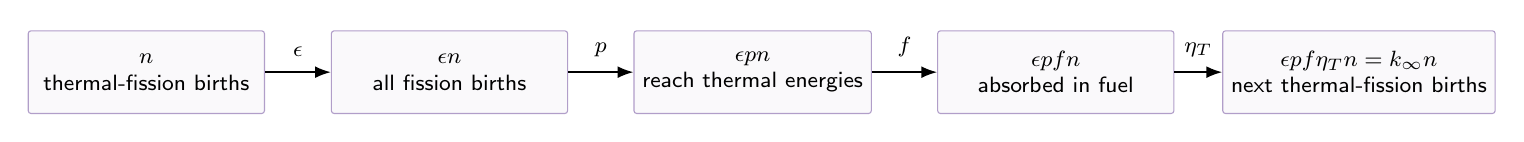
\begin{tikzpicture}[x=1cm,y=1cm,>=Latex,
 box/.style={draw=KSUPurple!45,fill=KSUPurple!3,rounded corners=1pt,
 minimum width=3.0cm,minimum height=1.05cm,align=center,inner sep=3pt},
 every node/.style={font=\sffamily\fontsize{8.2}{9.5}\selectfont}]
 \node[box] (n) at (0,0) {$n$\\thermal-fission births};
 \node[box] (en) at (3.85,0) {$\epsilon n$\\all fission births};
 \node[box] (epn) at (7.7,0) {$\epsilon p n$\\reach thermal energies};
 \node[box] (epfn) at (11.55,0) {$\epsilon p f n$\\absorbed in fuel};
 \node[box] (kn) at (15.4,0) {$\epsilon p f\eta_T n=k_\infty n$\\next thermal-fission births};
 \draw[->,line width=.6pt] (n)--(en) node[midway,above=2pt] {$\epsilon$};
 \draw[->,line width=.6pt] (en)--(epn) node[midway,above=2pt] {$p$};
 \draw[->,line width=.6pt] (epn)--(epfn) node[midway,above=2pt] {$f$};
 \draw[->,line width=.6pt] (epfn)--(kn) node[midway,above=2pt] {$\eta_T$};
\end{tikzpicture}}

% Qualitative Doppler/space-energy shielding sketch, adapted from Fig. 4.6.
\newcommand{\ResonanceFigure}{%
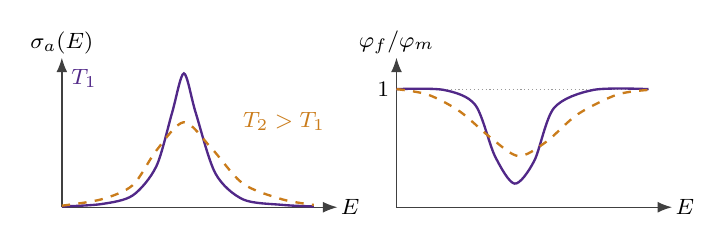
\begin{tikzpicture}[x=1cm,y=1cm,>=Latex,
 ax/.style={->,line width=.5pt,draw=black!75},
 cold/.style={line width=.85pt,draw=KSUPurple},
 hot/.style={line width=.85pt,draw=KSUOrange,dashed},
 every node/.style={font=\sffamily\fontsize{8.1}{9}\selectfont,inner sep=1pt}]
\begin{scope}
 \draw[ax] (0,0)--(3.5,0) node[right] {$E$};
 \draw[ax] (0,0)--(0,1.9) node[above] {$\sigma_a(E)$};
 \draw[cold] plot[smooth] coordinates {(0,.01)(.5,.04)(.9,.15)(1.2,.52)(1.4,1.2)(1.55,1.7)(1.7,1.2)(1.95,.43)(2.3,.10)(2.8,.03)(3.2,.01)};
 \draw[hot] plot[smooth] coordinates {(0,.02)(.5,.10)(.9,.28)(1.2,.72)(1.55,1.08)(1.9,.75)(2.3,.30)(2.8,.10)(3.2,.03)};
 \node[anchor=west,text=KSUPurple] at (.08,1.63) {$T_1$};
 \node[anchor=west,text=KSUOrange] at (2.26,1.09) {$T_2>T_1$};
\end{scope}
\begin{scope}[shift={(4.25,0)}]
 \draw[ax] (0,0)--(3.5,0) node[right] {$E$};
 \draw[ax] (0,0)--(0,1.9) node[above] {$\varphi_f/\varphi_m$};
 \draw[black!40,densely dotted] (0,1.5)--(3.2,1.5);
 \node[anchor=east] at (-.05,1.5) {$1$};
 \draw[cold] plot[smooth] coordinates {(0,1.5)(.6,1.49)(1,1.3)(1.25,.65)(1.5,.3)(1.75,.59)(2,1.26)(2.5,1.49)(3.2,1.5)};
 \draw[hot] plot[smooth] coordinates {(0,1.5)(.4,1.43)(.8,1.22)(1.2,.88)(1.55,.65)(1.9,.83)(2.3,1.18)(2.8,1.43)(3.2,1.49)};
\end{scope}
\end{tikzpicture}}
